% !TEX root = ../linal_lecture_05.tex

\begin{frame} % название фрагмента

\videotitle{Квадратичная форма}

\end{frame}



\begin{frame}{Краткий план:}
  \begin{itemize}[<+->]
    \item Определение квадратичной формы.
    \item Определённость формы.
  \end{itemize}

\end{frame}



\begin{frame}
    \frametitle{Квадратичная форма}    

    \begin{block}{Определение}
       Многочлен от нескольких переменных $f(x_1, x_2, \ldots, x_n)$, который содержит только слагаемые вида $x_i^2$ и $x_i x_j$ 
       \alert{квадратичной формой}.
    \end{block}

    \pause
    Функция $f(x,y) = x^2 + 6xy - 7y^2$ — квадратичная форма.

    \pause
    Функция $f(x, y, z) = x^2 + 6xz - 8xy + 3z + 9$ — не квадратичная форма. 
\end{frame}


\begin{frame}{Зачем нужны квадратичные формы?}
    
    Многие функции хорошо аппроксимируются суммой вида
    \[
    f(x, y) \approx 6 + 2x + 4y + 7x^2 + 8xy - 9y^2
    \]
    \pause
    Свойства квадратичной формы позволяют понять свойства многих функций!
    
\end{frame}


\begin{frame}{Квадратичная форма и матрицы}
\[
\begin{pmatrix}
    x_1 & x_2 & x_3 
\end{pmatrix} \cdot \begin{pmatrix}
    5 & \red{-1} & \blue{-3} \\
    \red{-1} & 7 & 2 \\
    \blue{-3} & 2 & 11 \\
\end{pmatrix} \cdot 
\begin{pmatrix}
    x_1 \\
     x_2 \\ 
     x_3 \\
\end{pmatrix} = \pause
\]
\[
 = 5x_1^2 + 7x_2^2 + 11x_3^2 \red{- 2}x_1 x_2 \blue{- 6}x_1 x_3 + 4 x_2 x_3 \pause
\]
    
\begin{block}{Утверждение}
    Любая квадратичная форма $f(\bx)$ может быть записана в виде 
    \[
      f(\bx) = \bx^T A \bx,  
    \]
    где $A$ — симметричная матрица, $A^T = A$.
\end{block}


\end{frame}


\begin{frame}
    \frametitle{Квадратичные формы в нуле}

    \begin{block}{Утверждение}
        Любая квадратичная форма $f$ равна $0$ в точке $\bzero$,
        \[
        f(\bzero)  = \bzero^T \cdot A \cdot \bzero = 0.
        \]
    \end{block}
    \pause
    Нас будет интересовать знак формы $f(\bx)$ при $\bx \neq \bzero$.

\end{frame}


\begin{frame}
    \frametitle{Положительно определённая форма}

    \begin{block}{Определение}
        Форма $f$ называется \alert{положительно определённой}, если $f(\bx) > 0$ при $\bx\neq\bzero$.
    \end{block}

    \pause

    \begin{center}
        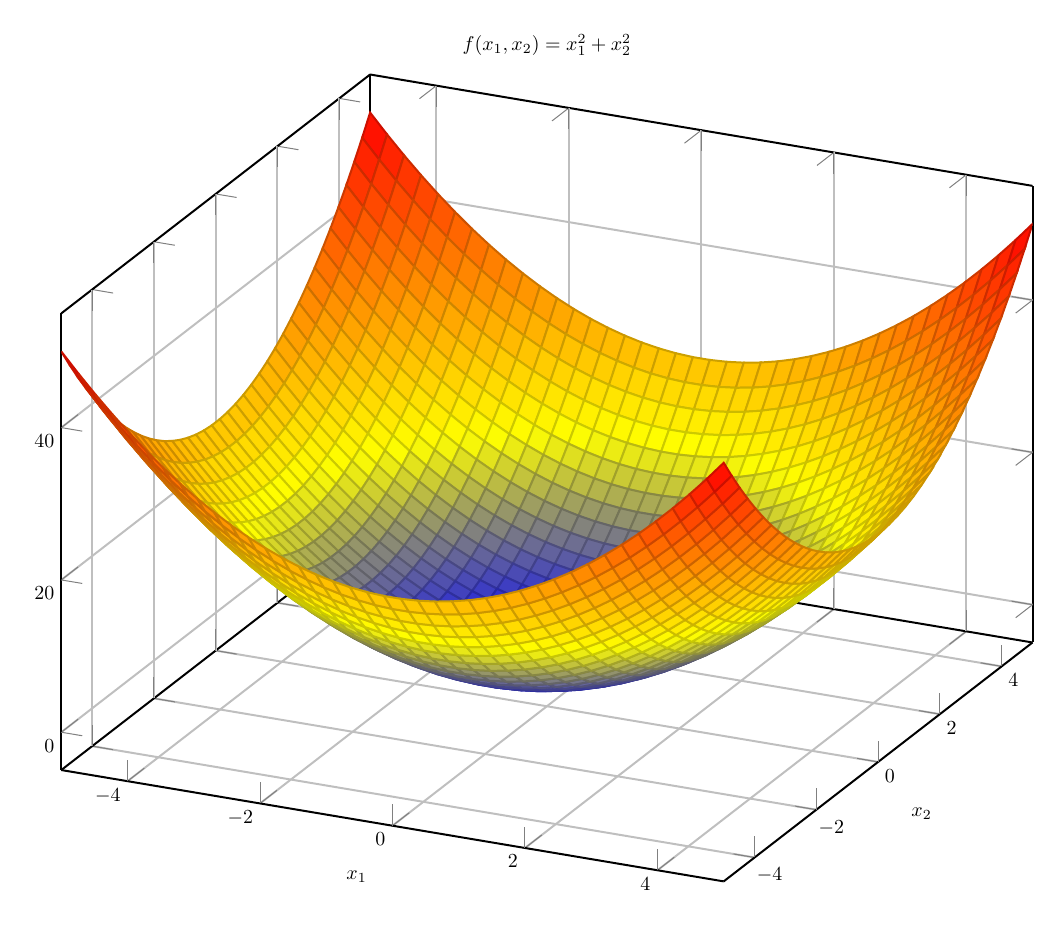
\begin{tikzpicture}[
        scale=1.8,
        every node/.style={scale=0.4}
        ]
        \begin{axis}[grid=both, title = {$f(x_1,x_2) = x_1^2+x_2^2$},xlabel = $x_1$, ylabel = $x_2$, xtick = {-4,-2,...,4},
        ytick = {-4,-2,...,4}]
        \addplot3[surf,shader=faceted, samples=40] {x^2+y^2};
        \end{axis}
        \end{tikzpicture}
    \end{center}
    
\end{frame}


\begin{frame}
    \frametitle{Отрицательно определённая форма}

    \begin{block}{Определение}
        Форма $f$ называется \alert{отрицательно определённой}, если $f(\bx) < 0$ при $\bx\neq\bzero$.
    \end{block}

    \pause

\begin{center}		
    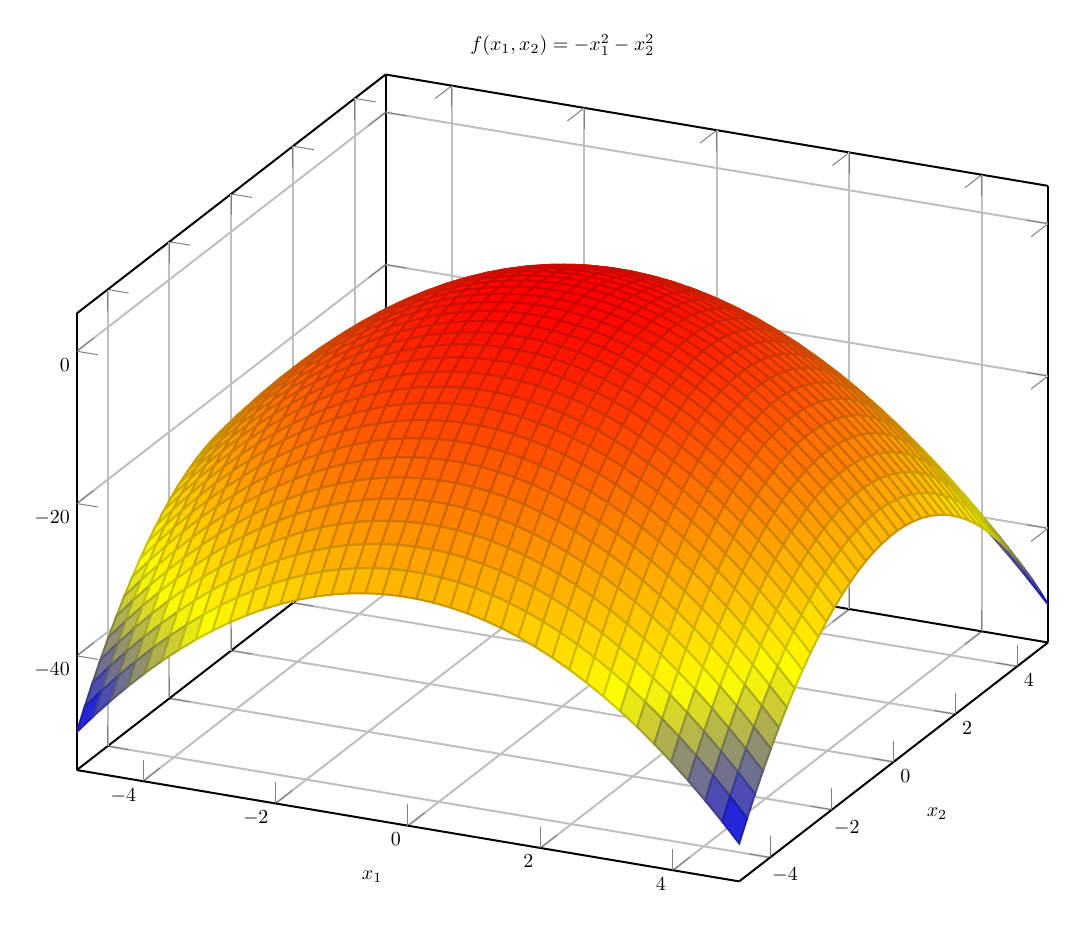
\begin{tikzpicture}[
    scale=1.8,
    every node/.style={scale=0.4}
    ]
    \begin{axis}[grid=both, title = {$f(x_1,x_2) = -x_1^2-x_2^2$}, xlabel = $x_1$, ylabel = $x_2$, xtick = {-4,-2,...,4},
    ytick = {-4,-2,...,4}]
    \addplot3[surf,shader=faceted, samples=40] {-x^2-y^2};
    \end{axis}
    \end{tikzpicture}
\end{center}
    
\end{frame}



\begin{frame}
    \frametitle{Положительно полуопределённая форма}

    \begin{block}{Определение}
        Форма $f$ называется \alert{положительно полуопределённой} или
        \alert{неотрицательно определённой}, если $f(\bx) \geq 0$.
    \end{block}

    \pause

\begin{center}
    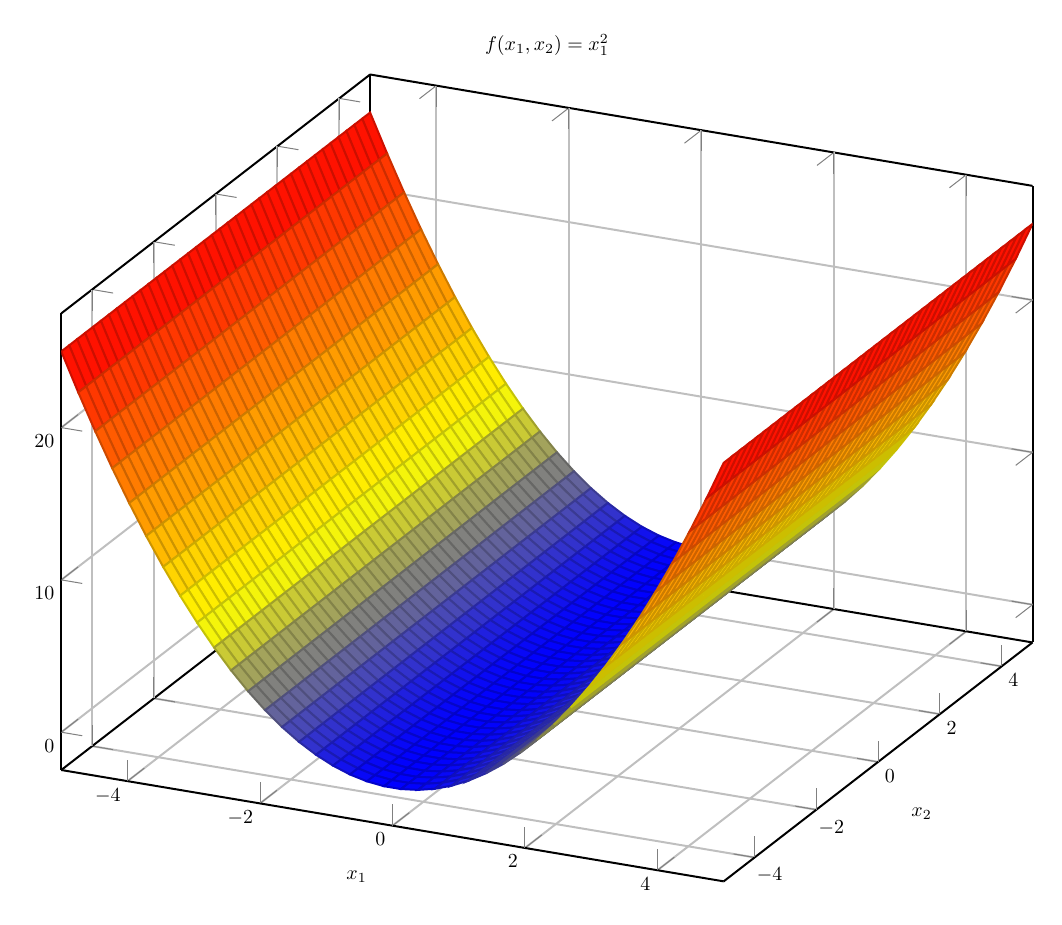
\begin{tikzpicture}[
    scale=1.8,
    every node/.style={scale=0.4}
    ]
    \begin{axis}[grid=both, title = {$f(x_1,x_2) = x_1^2$}, xlabel = $x_1$, ylabel = $x_2$, xtick = {-4,-2,...,4},
    ytick = {-4,-2,...,4}]
    \addplot3[surf,shader=faceted, samples=40] {x^2};
    \end{axis}
    \end{tikzpicture}
\end{center}
    
\end{frame}



\begin{frame}
\frametitle{Отрицательно полуопределённая форма}

\begin{block}{Определение}
    Форма $f$ называется \alert{отрицательно полуопределённой} или
    \alert{неположительно определённой}, если $f(\bx) \leq 0$.
\end{block}

    \pause

\begin{center}
    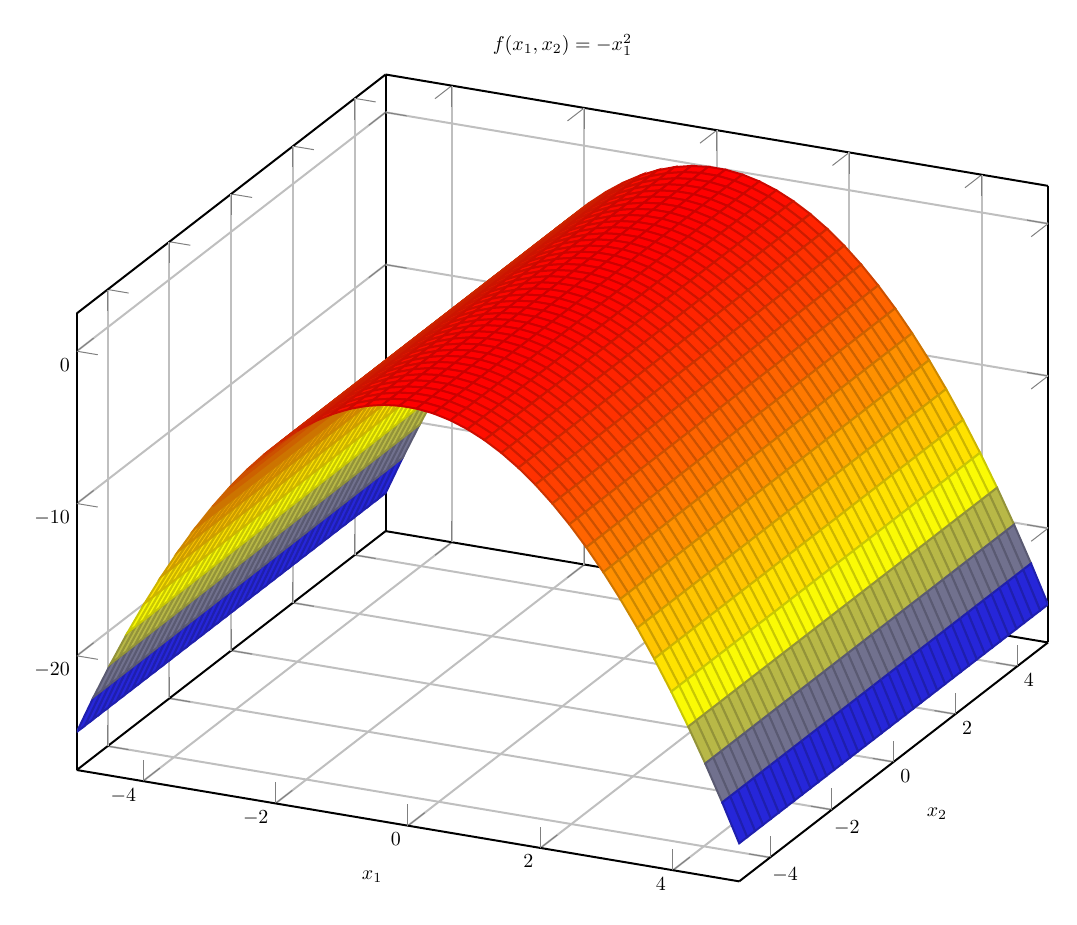
\begin{tikzpicture}[
    scale=1.8,
    every node/.style={scale=0.4}
    ]
    \begin{axis}[grid=both, title = {$f(x_1,x_2) = -x_1^2$},xlabel = $x_1$, ylabel = $x_2$, xtick = {-4,-2,...,4},
    ytick = {-4,-2,...,4}]
    \addplot3[surf,shader=faceted, samples=40] {-x^2};
    \end{axis}
    \end{tikzpicture}
\end{center}
    
\end{frame}



\begin{frame}
    \frametitle{Неопределённая форма}

    \begin{block}{Определение}
        Форма $f$ называется \alert{неопределённой}, если она принимает и положительные и отрицательные значения.
    \end{block}

    \pause

\begin{center}
    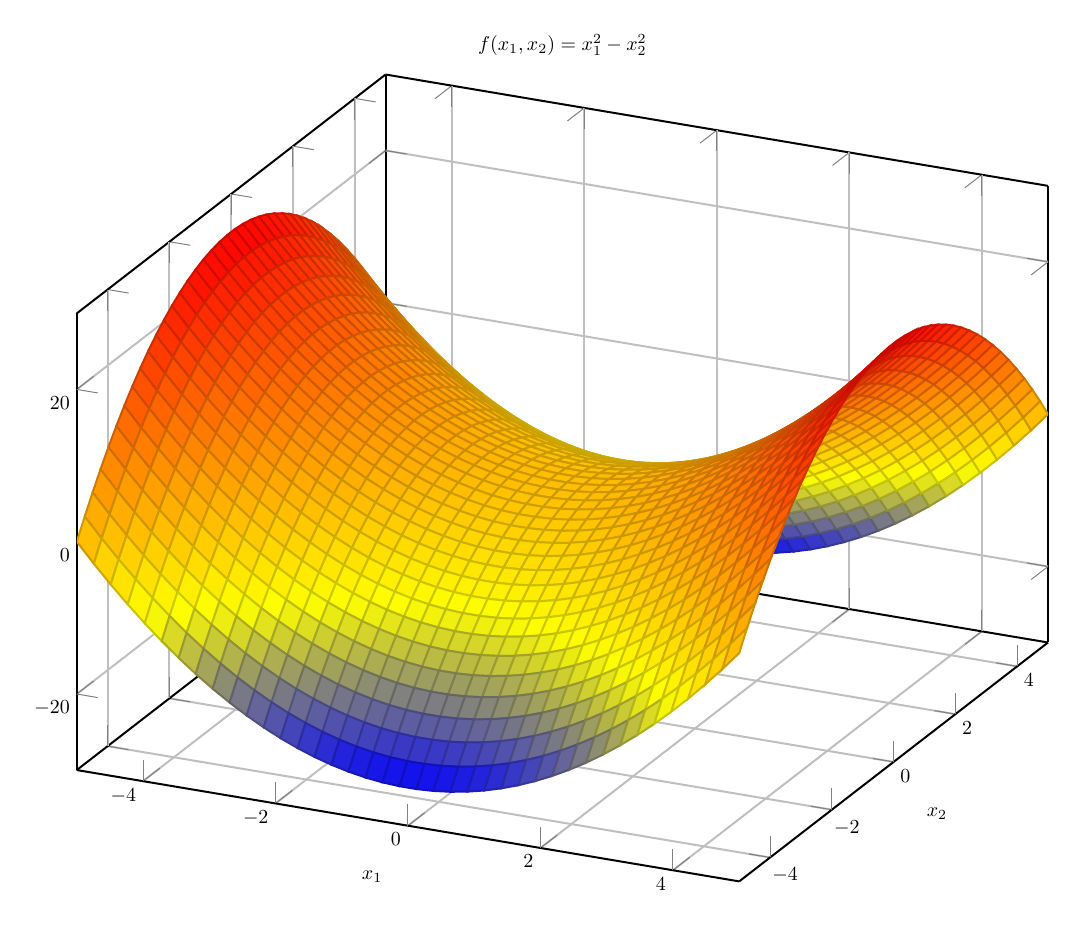
\begin{tikzpicture}[
    scale=1.8,
    every node/.style={scale=0.4}
    ]
    \begin{axis}[grid=both, title = {$f(x_1,x_2) = x_1^2-x_2^2$},xlabel = $x_1$, ylabel = $x_2$, xtick = {-4,-2,...,4},
    ytick = {-4,-2,...,4}]
    \addplot3[surf,shader=faceted, samples=40] {x^2-y^2};
    \end{axis}
    \end{tikzpicture}
\end{center}
    
\end{frame}



\begin{frame}
    \frametitle{Когда форма равна нулю?}

    \begin{block}{Утверждение}
        Если форма $f$ равна $0$ в точке $\bx$, то она равна нулю и
        в любой точке $t\bx$. 
    \end{block}
    \pause
    \begin{block}{Доказательство}
        \[
        f(t\bx) = t\bx^T \cdot A \cdot t\bx = t^2 \bx^T A \bx = 0
        \]
    \end{block}
    \pause
    Квадратичная форма возможно равна нулю на прямых, проходящих через $\bzero$.
    
\end{frame}